\chapter{Initial Dataset Creation}\label{ch:datasetCreation}

Before the development of an automated photo-id aid could begin, the procurement of large scale data with a distribution similar to that seen during photo-id surveys was required. Exploration of available open-source datasets to find images of cetaceans in similar conditions to those seen in photo-id survey data proved unfruitful. Many standard benchmarking datasets contain animal classes, and thus an exploration of these was conducted. Of the more generalised benchmark datasets, those such as ImageNet \cite{deng_imagenet:_2009} which contain a large corpus of varied classes, only CIFAR-100 \cite{krizhevsky_learning_2009} contains a \texttt{dolphin} class. However, images in CIFAR-100 are only 32x32 pixels in size, too small to be useful for the task at hand. 

Moving the search away from generalised datasets and towards those which are targeted at conservation efforts or the natural environment also proved fruitless. A large portion of these datasets focus on camera traps or land-based fauna, such as iWildCam \cite{beery_iwildcam_2019}, for reasons discussed in more detail in Section \ref{ch:Background,sec:conTech}. Some images included in the iNaturalist dataset \cite{van_horn_inaturalist_2018} are of cetaceans, such as a class for the short-beaked common dolphin (\textit{Delphinus delphis}), however most focus on other aquatic animals such as the Florida manatee (\textit{Trichechus manatus}), various amphibians, and molluscs. 

As no open-source image datasets containing the data required for the work in this thesis were available, this chapter outlines the work undertaken to develop these. The creation of a coarse-grained instance segmentation dataset consisting of readily available survey data collected around the waters of Zanzibar, Tanzania is first discussed. Next, the creation of a dataset consisting of data collected around the waters of Northumberland, UK, known as the Northumberland Dolphin Dataset 2020 (NDD20)\nomenclature[z-NDD20]{NDD20}{Northumberland Dolphin Dataset 2020}, is discussed. This dataset contains coarse-grained instance segmentation data, as well as fine-grained species and individual level data. 

\section{The Zanzibar Dataset}\label{ch:datasetCreation,sec:zanzibar}

Due to the lack of open-source datasets to aid in the development of the cetacean detector, a photo-id catalogue curated during a 2015 research effort undertaken in Zanzibar, Tanzania by Newcastle University's Marine MEGAfauna Lab was obtained. This catalogue was utilised to determine the status of Indo-Pacific bottlenose dolphins (\textit{Tursiops aduncus}) in the area \cite{sharpe_indian_2019}, and consisted of 1021 images of size 5184x3456 -- supplied in a format suitable for manual photo-identification rather than for the training of a neural network. Work was then undertaken to convert this catalogue into a machine learning dataset. 

In order to perform this conversion, the provided images were first labelled. This was achieved using the VGG Image Annotator software (VIA) \cite{dutta_via_2019}. Other labelling software such as LabelImg \cite{tzutalin_labelimg_2021} was examined, however VIA was deemed the best choice for the task at hand. This software was chosen for multiple reasons; first, the software is noticeably easy to use and allows for efficient labelling on a per-pixel basis as required by Mask R-CNN. Second, the tutorial data provided by the Mask R-CNN Github repository was labelled in VIA format, showing that this code implementation would accept data labelled in this format. Furthermore, use cases of VIA being utilised for labelling of marine-oriented data are available in the literature \cite{nita_cnn-based_2020}, providing evidence of suitability of the labelling software for research purposes and data representing similar conditions.

Before labelling the Zanzibar data, some curation was performed. Each image labelled by VIA is required to contain at least one non-background class. As such, any images provided which did not contain an example of a \texttt{dolphin} class were discarded. Other images where the class examples were unsuitable for training a Mask R-CNN model, such as those which contained only an extremely small section of the photographed dolphin or were deemed too blurry, were also removed. This left 312 images which were suitable for the Mask R-CNN.

The process for labelling the data with VIA is rather straightforward. The software runs locally through a web browser, with each image labelled sequentially. Figure \ref{fig:via-json-example-zanzibar} shows an example image labelled using VIA. Each image is shown on-screen to the user who is then able to trace around class examples by selecting multiple points on the image. Once a full trace has been performed, any pixels inside of the trace are treated as one class. This class is labelled through the use of a class attribute, in the case of the Zanzibar data this was the class label \texttt{dolphin}, denoting the class example as an animal breaching the waterline. These labels are stored in a corresponding JSON file, which is fed to the Mask R-CNN model along with the images during training. This labelling allows the model to learn per-pixel class examples during training. This tracing method also allows for each distinct individual in a group to be labelled individually, even if overlapping, which would be much harder to perform with bounding box labelling and allows the model to learn how to differentiate between group members.  

\begin{figure}
	\begin{center}
		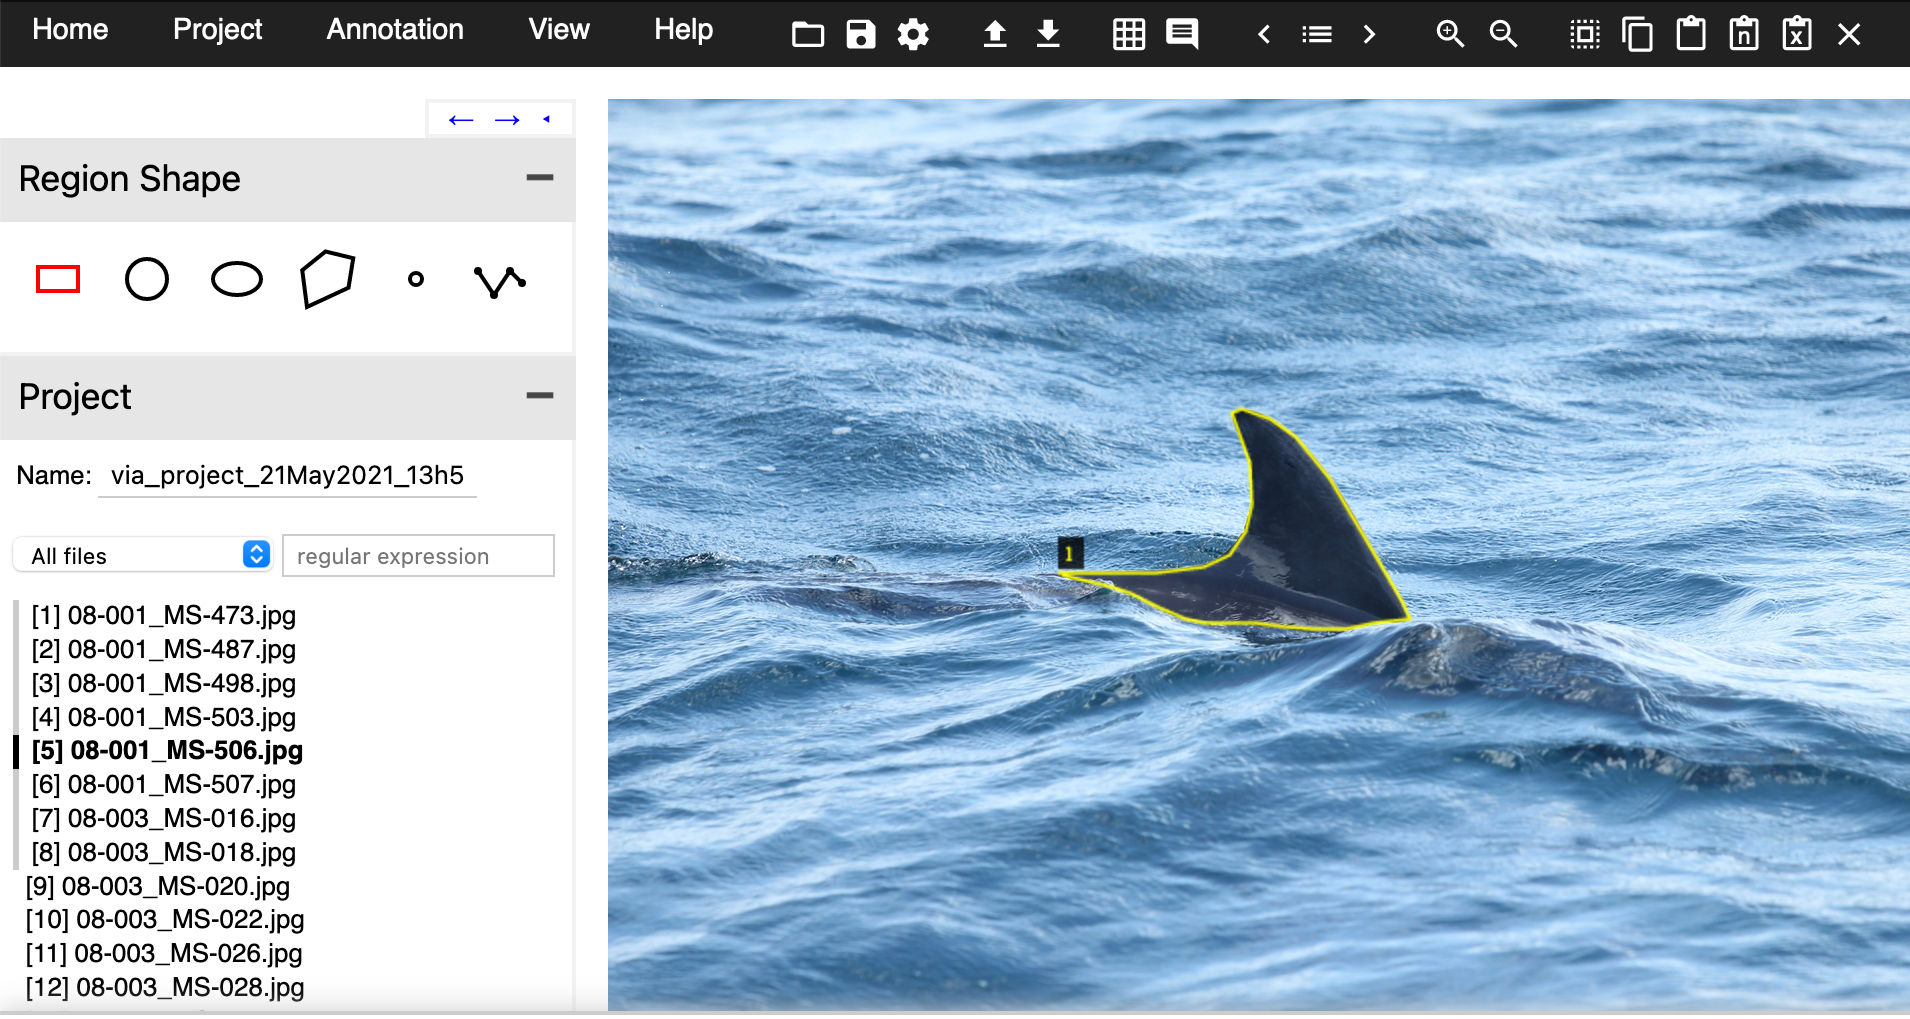
\includegraphics[width=\linewidth]{Chapter3/figs/via-json-example-zanzibar-1-updated.png}
	\end{center}
	\caption[An example of the labelling process using VIA.]{An example of labelling process using VIA. The dorsal fin in the image selected has been traced, highlighted by the yellow outline.
	}
	\label{fig:via-json-example-zanzibar}
\end{figure}

\section{The Northumberland Dolphin Dataset 2020}\label{ch:datasetCreation,sec:NDD}

Whilst the creation of the Zanzibar dataset allows for the development of a model capable of coarse-grained automated detection of cetaceans from photo-id imagery, as no fine-grained individual IDs are present it does not contain the information required to allow for the training of a model capable of individual identification. As a result, this section discusses the collection of abundance estimate data off the coast of Northumberland, UK. The collected photo-identification data was then curated and transformed from an ecological catalogue into a fine-grained computer vision dataset known as The Northumberland Dolphin Dataset 2020 (NDD20), to allow for the development of an automated catalogue matching system to occur. 

Surveys undertaken and described within this section also provided data for two other theses at Newcastle University, one within the School of Electrical and Electronic Engineering focussing on the automated identification of cetaceans via signature whistles and the other within the School of Natural and Environmental Sciences focussing on the creation of abundance and health assessments of the cetaceans resident in the survey area.

\subsection{Data Collection}\label{ch:datasetCreation,sec:NDD,sub:dataCollection}

The following section provides context for the data collection survey, beginning by briefly outlining the geographic area in which the data was collected and discussion of why the area was chosen. Next the survey effort is discussed in detail, including a run-down of the methodology used, for the purposes of reproducibility. 

\subsection{The Survey Area}\label{ch:datasetCreation,sec:NDD,sub:surveyArea}

Whilst the Marine MEGAfauna Lab conducts research heavily in the Indian Ocean around Zanzibar \cite{yang_description_2020, temple_life-history_2020, temple_marine_2019, temple_marine_2018, weigmann_revision_2020, barrowclift_social_2017}, this is not the only place they operate \cite{temple_by-catch_2021, yang_classification_2017, yang_influence_2022}. In recent years, their work has begun to include more local waters such as the North Sea off the coast of Northumberland, UK \cite{van_bressem_visual_2018, yang_characterization_2021}. These waters are known to host a wide variety of marine mammals, with the Marine MEGAfauna Lab focussing efforts specifically on the common bottlenose dolphin (\textit{Tursiops truncatus}) and white-beaked dolphin (\textit{Lagenorhynchus albirostris}) populations. 

Data collection was conducted in and around the Coquet to St. Mary's Marine Conservation Zone (MCZ)\nomenclature[z-MCZ]{MCZ}{Marine Conservation Zone}, located off the coast of Northumberland, UK. The MCZ, established in January 2016 through powers granted by the Marine and Coastal Access Act 2009 \cite{noauthor_marine_2009}, covers approximately 40km of coastline from Alnmouth in the north to Whitley Bay in the south, extending outwards 7.5km at its greatest to cover an area around 192km$^{2}$. A map of the survey area and MCZ can be seen in Figure \ref{fig:survey-map}.

 \begin{figure}
	\begin{center}
		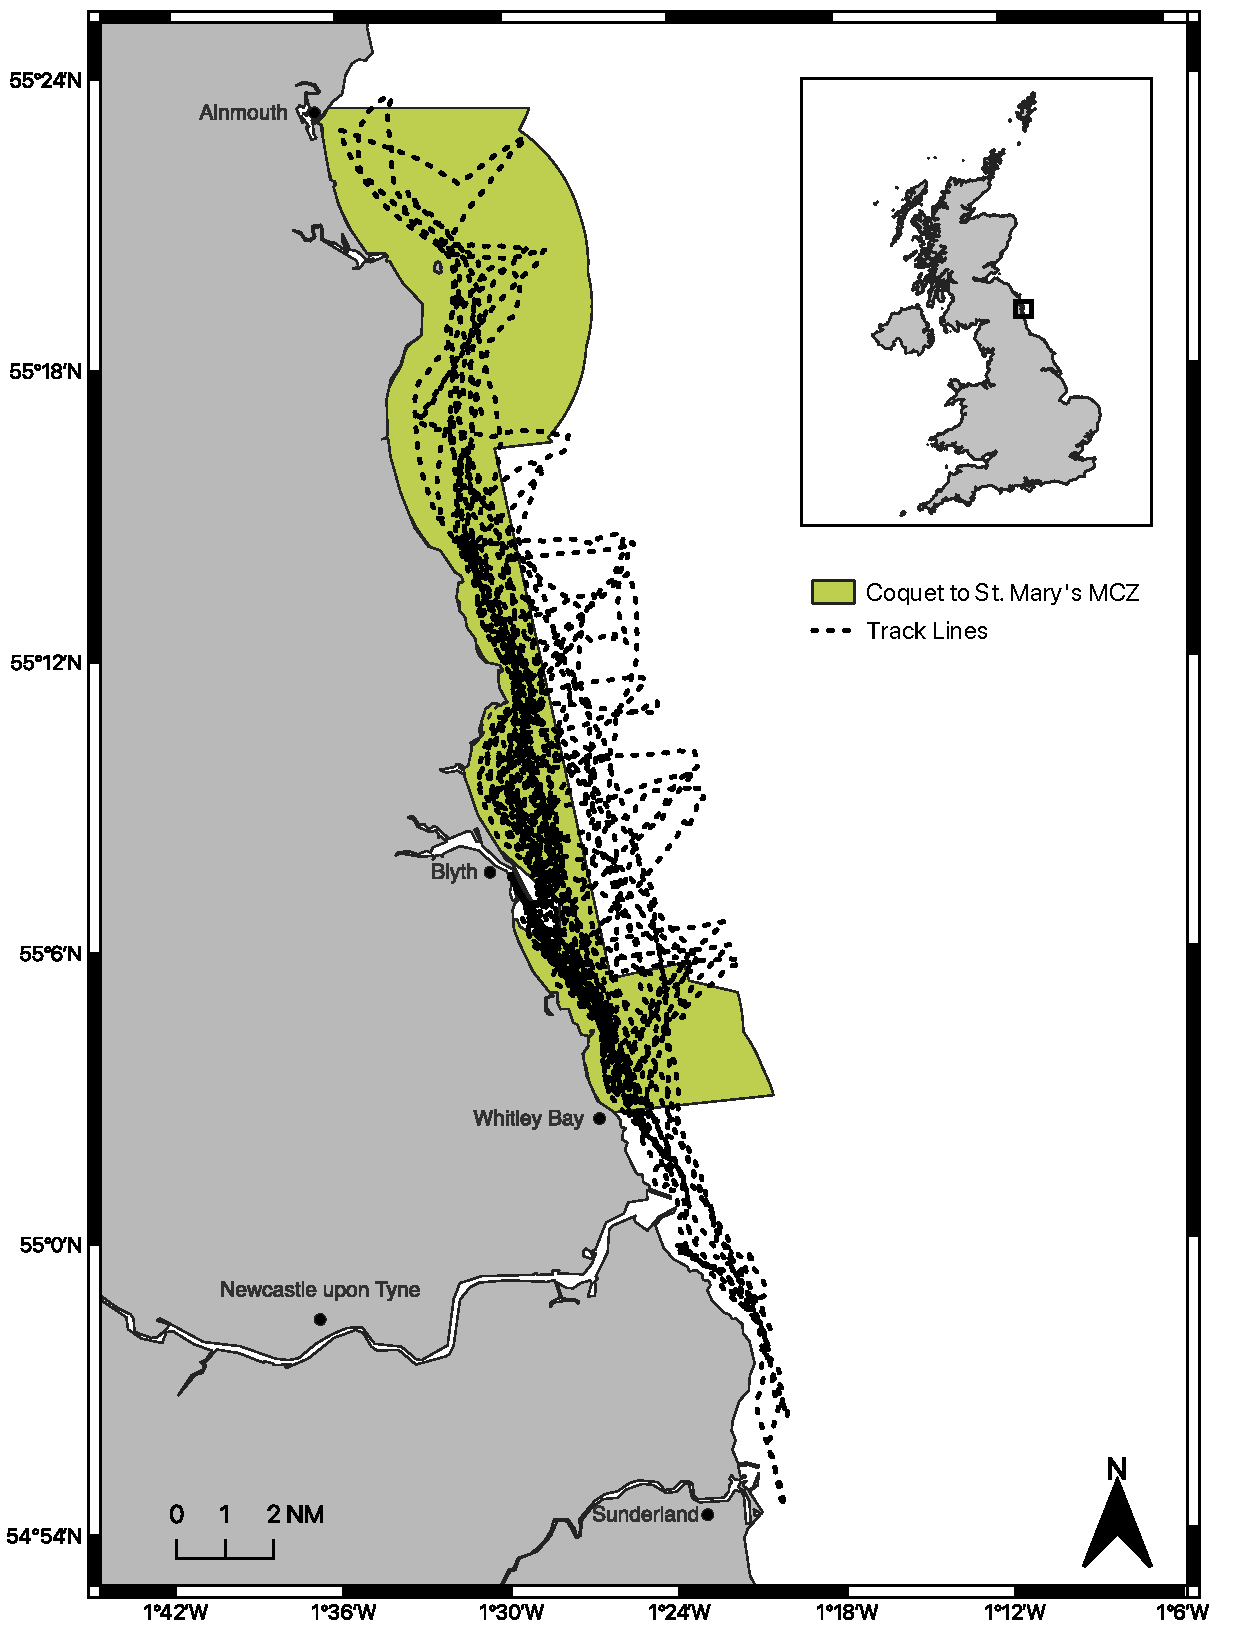
\includegraphics[scale=0.7]{Chapter3/figs/survey_map.pdf}
	\end{center}
	\caption[Map of the survey area, with the Coquet to St. Mary's MCZ highlighted.]{Map of the survey area, with the Coquet to St. Mary's MCZ highlighted. Track lines for all survey days are overlaid.}
	\label{fig:survey-map}
\end{figure}

The area is of high ecological importance, supporting a wide variety of marine life thanks to sections of intertidal and sub-tidal rock and sediment, making it fertile feeding grounds for the bottlenose and white-beaked dolphins which make use of the area. As a result of this fertility, as well as waters up to 30m deep in some places, the MCZ sees high levels of fishing activity -- typically for crustaceans using pots \cite{stephenson_spatial_2017}. Whilst these fishing vessels operate from a number of small ports throughout the North East of England, the MCZ itself lies close to the large Port of Blyth. As a result, the MCZ boundary provides a 250m buffer zone around the limits of the port in order to reduce economic damage. This survey region was selected as no previous surveying had been undertaken in the area for the purposes of cetacean abundance estimates and health assessment.  

\subsection{Survey Effort}\label{ch:datasetCreation,sec:NDD,sub:surveyEffort}

Dedicated bottlenose and white-beaked dolphin photo-identification surveys were conducted in the MCZ between 19/07/2019 and 10/10/2019, with a total of 27 surveys undertaken. These were performed using a 5.6m rigid inflatable boat (RIB)\nomenclature[z-RIB]{RIB}{Rigid Inflatable Boat} with a 50 horsepower four-stroke outboard engine. All surveys began from Newcastle University's Blyth Marine Station, located in the Port of Blyth, before entering the MCZ.

Surveys initially began by following set transect lines, traversing between the northern and southern-most points of the MCZ. Thanks to limited success encountering individuals strictly following transect lines however, the survey switched to more opportunistic surveying based on reports from two citizen science groups: the Newbiggin-by-the-Sea Dolphin Watch\footnote{Newbiggin-by-the-Sea Dolphin Watch: \href{https://en-gb.facebook.com/groups/NEWILDDOLPHINMONITORINGPROJECT/}{facebook.com/groups/NEWILDDOLPHINMONITORINGPROJECT}} and the North East Cetacean Project\footnote{North East Cetacean Project: \href{https://en-gb.facebook.com/groups/NorthEastCetaceanProject/about/}{facebook.com/groups/NorthEastCetaceanProject}}. The use of citizen scientists for photo-id surveys has seen increased prevalence in recent years, with multiple studies producing promising results if access to groups of dedicated citizen scientists is available, as in Northumberland \cite{araujo_population_2017, currie_conservation_2018, armstrong_photographic_2019, araujo_photo-id_2019}. Track lines showing movement of the vessel were recorded via GPS tracking, and can be seen in Figure \ref{fig:survey-map}. When dolphins were encountered, the time stamp was recorded alongside other effort data such as direction of travel, sea state, species, group size, and demographic composition.

Surveys were only conducted in Beaufort Sea States $<4$ \cite{world_meteorologicial_society_beaufort_1970} without heavy rain. Outside of these conditions surveying can become unsafe and the photographs unusable for photo-id because of swell and lens splash. Due to the nature of the North Sea, conditions outside of these restrictions can be common. Surveying was performed using the constant scanning method \cite{mann_behavioral_1999}, with cues including sight of dorsal fins breaching the waterline, splashing, and leaping. For each survey the vessel was manned by at least two dedicated observers and a skipper, in line with other photo-id surveys \cite{sharpe_indian_2019, bessesen_lacaziosis-like_2014, silva_winter_2012}.

Individual dolphins in an encounter were photographed randomly using a Canon EOS 550D Digital SLR with a Canon 70–200mm zoom lens, aiming to capture photographic data for every individual present. Camera settings can be found in Appendix \ref{app:DataCollectionCameraSettings}. Multiple photographs were captured of each cetacean over the course of the encounter to ensure identifiable information could be fully captured. 

When capturing an encounter care was taken not to approach individual cetaceans at an angle less than $30^{\circ}$, keeping as parallel as possible and to speeds no greater than 6 knots in order to prevent the cetaceans becoming stressed or injured as per Marine Management Organisation guidelines. All members of the survey team were trained in minimising wildlife disturbance through the WiSe Scheme by the Yorkshire Wildlife Trust\footnote{WiSe Scheme: \href{https://www.wisescheme.org/}{wisescheme.org}}, with the survey itself having the approval of Newcastle University's Ethics Board.

\subsection{Field Season Summary}\label{ch:datasetCreation,sec:NDD,sub:FieldSeasonSummary}

In total, 27 surveys were conducted with 14 containing encounters. Of these, 12 were made up of bottlenose dolphins; only two were made up of white-beaked dolphins. No encounters contained both species. Groups were defined using the 10m chain rule \cite{smolker_sex_1992}. Group size averaged 12 for bottlenose dolphins, typical for the species \cite{shane_ecology_1986}. Altogether 44 individuals were identified and catalogued, broken down into 30 bottlenose and 10 white-beaked dolphins. Of all animals encountered, 27\% were calves. They have been excluded from this analysis as they could not be considered independent due to reliance on their mothers, and had not yet developed permanent markings.

Images collected were processed for use in the photo-identification catalogue to remove any images with no value, such as those which were out of focus or did not contain any cetacean. Animals present in the images were coded according to their distinctiveness as per the guidelines presented by Urian \textit{et al.} \cite{urian_recommendations_2015}. Those coded D1 were considered very distinctive with little chance of misidentification, whilst those coded D2 were considered moderately distinctive with small prominent markings which could allow for a high chance of correct classification provided the image is clear. CF coded individuals were those that contained little to no identifying information and have a high chance of misclassification. Once coded, animals considered D1 and D2 were individually identified.

\section{Creation of NDD20}\label{ch:datasetCreation,sec:NDD20}

The fieldwork season and data processing undertaken resulted in a photo-identification catalogue of bottlenose and white-beaked dolphins currently inhabiting the Coquet to St. Mary's MCZ. Photo-identification catalogues utilised in marine ecology however are not in the form required for training or validating a computer vision model. As such, further processing was required to transform the catalogue into a dataset capable of both validating the instance segmentation model developed in Chapter \ref{ch:cetDet}, as well as training a model for fine-grained individual identification. This section discusses the creation of the Northumberland Dolphin Dataset 2020 (NDD20) \cite{trotter_ndd20_2020}, the computer vision dataset created from the photo-identification catalogue collected in the MCZ.

\subsection{Above Water Data}\label{ch:datasetCreation,sec:NDD20,sub:aboveWaterData}

During fieldwork 4940 images were collected which contained part of a cetacean above the water line. Of these, 2201 images were considered usable for the creation of NDD20. Issues rendering images unusable included a significant amount of water splash obscuring the cetacean, poor lighting conditions, or where individuals in a pod were too close together to accurately determine by eye the outline of all individuals. 

From manual analysis it was determined that not all images contained enough identifying information for individual classification labels. Because of this, the decision was made to include multiple levels of granularity to the dataset. As all images contained part of a cetacean, each one could be labelled to allow for instance segmentation training. To enable this, each mask located was given the label \texttt{dolphin}. Next, masks could be provided a fine-grained species classification. Thanks to the difference in colour between bottlenose and white-beaked dolphins, every mask labelled for instance segmentation could also be provided a species label -- either \texttt{BND} or \texttt{WBD} representing bottlenose and white-beaked dolphin respectively. 

At the highest level of granularity, some masks contained enough information to allow for individual identification. If an ID could be attained with high confidence, likely from images with D1 or D2 coded individuals, the mask containing the individual was provided an \texttt{ID} label. Recent work has shown that publicly available datasets containing animals may aid poachers \cite{beery_can_2021}. In response, to protect ongoing cetacean research efforts a pseudo-anonomisation has been performed. This however does not diminish the value of the dataset to computer vision researchers. It is not the case that images with sequential filenames were captured sequentially, and all individual IDs have been randomly allocated a numerical value rather than the code given to them by the Marine MEGAfauna Lab. All EXIF data found in the images has also been removed.

Data was labelled at a pixel level using the VGG Image Annotator \cite{dutta_via_2019} in a similar fashion to the Zanzibar dataset as discussed in Section \ref{ch:datasetCreation,sec:zanzibar}. In order to speed up the process data labellers were employed through Newcastle University's Jobs On Campus service\footnote{Newcastle University Jobs On Campus: \href{https://www.ncl.ac.uk/careers/jobs/opportunities-on-campus/jobsoc/\#jobsocoverview}{ncl.ac.uk/careers/jobs/opportunities-on-campus/jobsoc/}} to manually annotate the masks and label them for instance segmentation. Once complete all masks were checked for error correcting and consistency purposes. Afterwards, the extra labels for both species and individual level identification were added. As this required expert knowledge, data labellers were not utilised for this. Example above water images from NDD20 and the labels assigned can be seen in Figure \ref{fig:above-water-example}.

\begin{figure}
	\begin{center}
		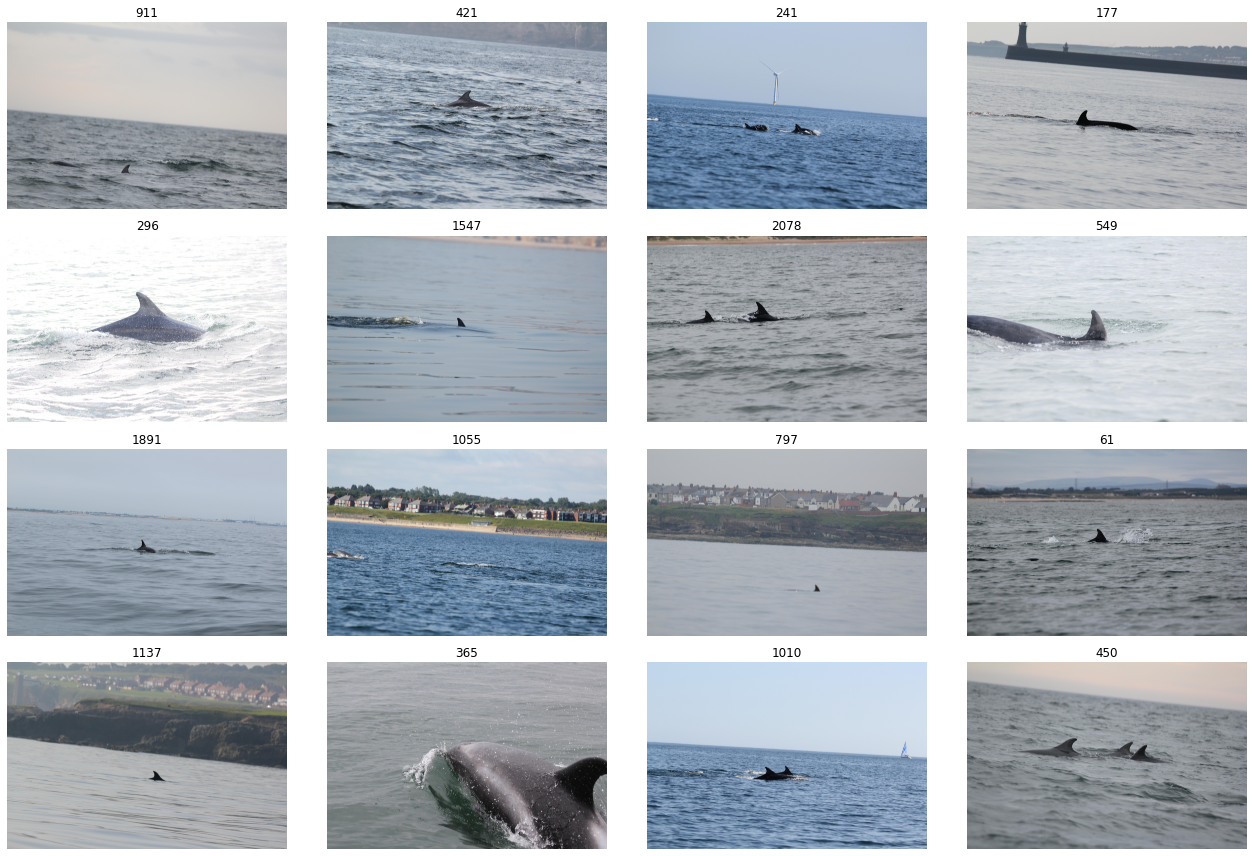
\includegraphics[scale=0.3]{Chapter3/figs/aweg-tiled.png}
	\end{center}
	\caption[Example above water images from NDD20 with filenames displayed.]{Example above water images from NDD20 with filenames displayed. Class labels for masks in each image are noted in Appendix \ref{app:NDD20AwegLabels}.}
	\label{fig:above-water-example}
\end{figure}

\subsection{Below Water Data}\label{ch:datasetCreation,sec:NDD20,sub:belowWaterData}

In addition to the above water imagery captured during fieldwork, NDD20 also contains below water images. Underwater photo-id is not as widely used compared to its above-water counterpart at present, however uses have been noted for certain species and environments in recent years \cite{van_bressem_visual_2018, veronique_underwater_2022}. Whilst this data has not been utilised in the work on automatic photo-id presented in this thesis it is important to discuss all aspects of the dataset created. Images contained in the below water section of NDD20 are a subset of a much larger collection of images produced by the Marine MEGAfauna Lab during work in the Farnes Deep MCZ, a glacial trench situated approximately 11km from the Northumberland coast. Opportunistic surveys undertaken since 2011 have shown the area to contain a high abundance of white-beaked dolphin activity \cite{van_bressem_visual_2018}. Data from these surveys takes the form of screen grabs from high definition video footage captured by a diver using GoPro Hero 3 and Go Pro Hero 4 cameras. 

To mirror the above water section, there are 2201 below water images included in NDD20 labelled for multiple levels of granularity. As before, the first attribute level is \texttt{dolphin} to allow for instance segmentation. Unlike the above water images, all below water images contain at least one mask with an \texttt{ID} label. It is not the case that masks in the above and below image sets contain the same individual animal even if they have the same \texttt{ID} class label -- the numbering systems are independent of one another. No species label is provided as all images are of white-beaked dolphins. Below water images are also labelled with an \texttt{out of focus} flag, denoting if the individual is deemed to be out of focus. Example below water images from NDD20 can be seen in Figure \ref{fig:below-water-example}.

\begin{figure}
	\begin{center}
		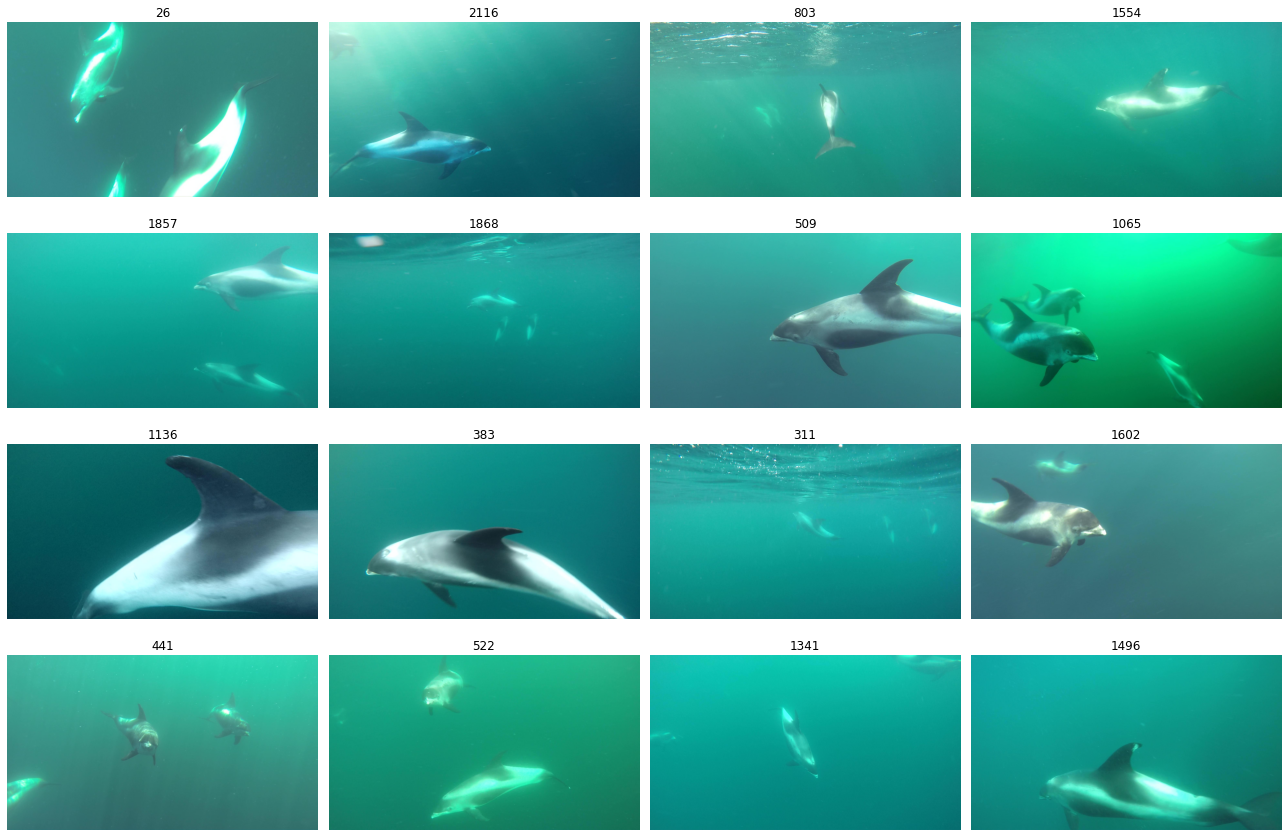
\includegraphics[scale=0.3]{Chapter3/figs/bweg-tiled.png}
	\end{center}
	\caption[Example below water images from NDD20 with filenames displayed.]{Example below water images from NDD20 with filenames displayed. Class labels for masks in each image are noted in Appendix \ref{app:NDD20BwegLabels}.}
	\label{fig:below-water-example}
\end{figure}

\subsection{NDD20 Summary}\label{ch:datasetCreation,sec:NDD20,sub:NDD20Summary}

As NDD20 is split into two related but distinct sets of images, a summary is provided below for each. Due to the nature of cetacean group dynamics, multiple images contain more than one individual animal. As a result, there are 2900 masks present in the above water set of 2201 images. These masks contain both a \texttt{dolphin} label for instance segmentation as well as either a \texttt{BND} or \texttt{WBD} label to facilitate species level fine-grained classification. It should be noted however that the distribution of species class labels is imbalanced, with 73\% of masks being labelled \texttt{BND}. Some above water masks also contain an individual level \texttt{ID} label to allow for extreme fine-grained classification. Due to the nature of the task only 14\% of masks contain an \texttt{ID} class label, with 44 distinct individuals present. Once again these classes are imbalanced presenting both a fine-grained and few-shot learning problem. The above water \texttt{ID} class label distribution can be seen in Figure \ref{fig:above-water-id-dist}. Many of the challenges associated with manual above water photo-id apply here too, particularly the likelihood that unique features are specific to one side of an animal's body which may not have been captured in the image.

\begin{figure}
	\begin{center}
		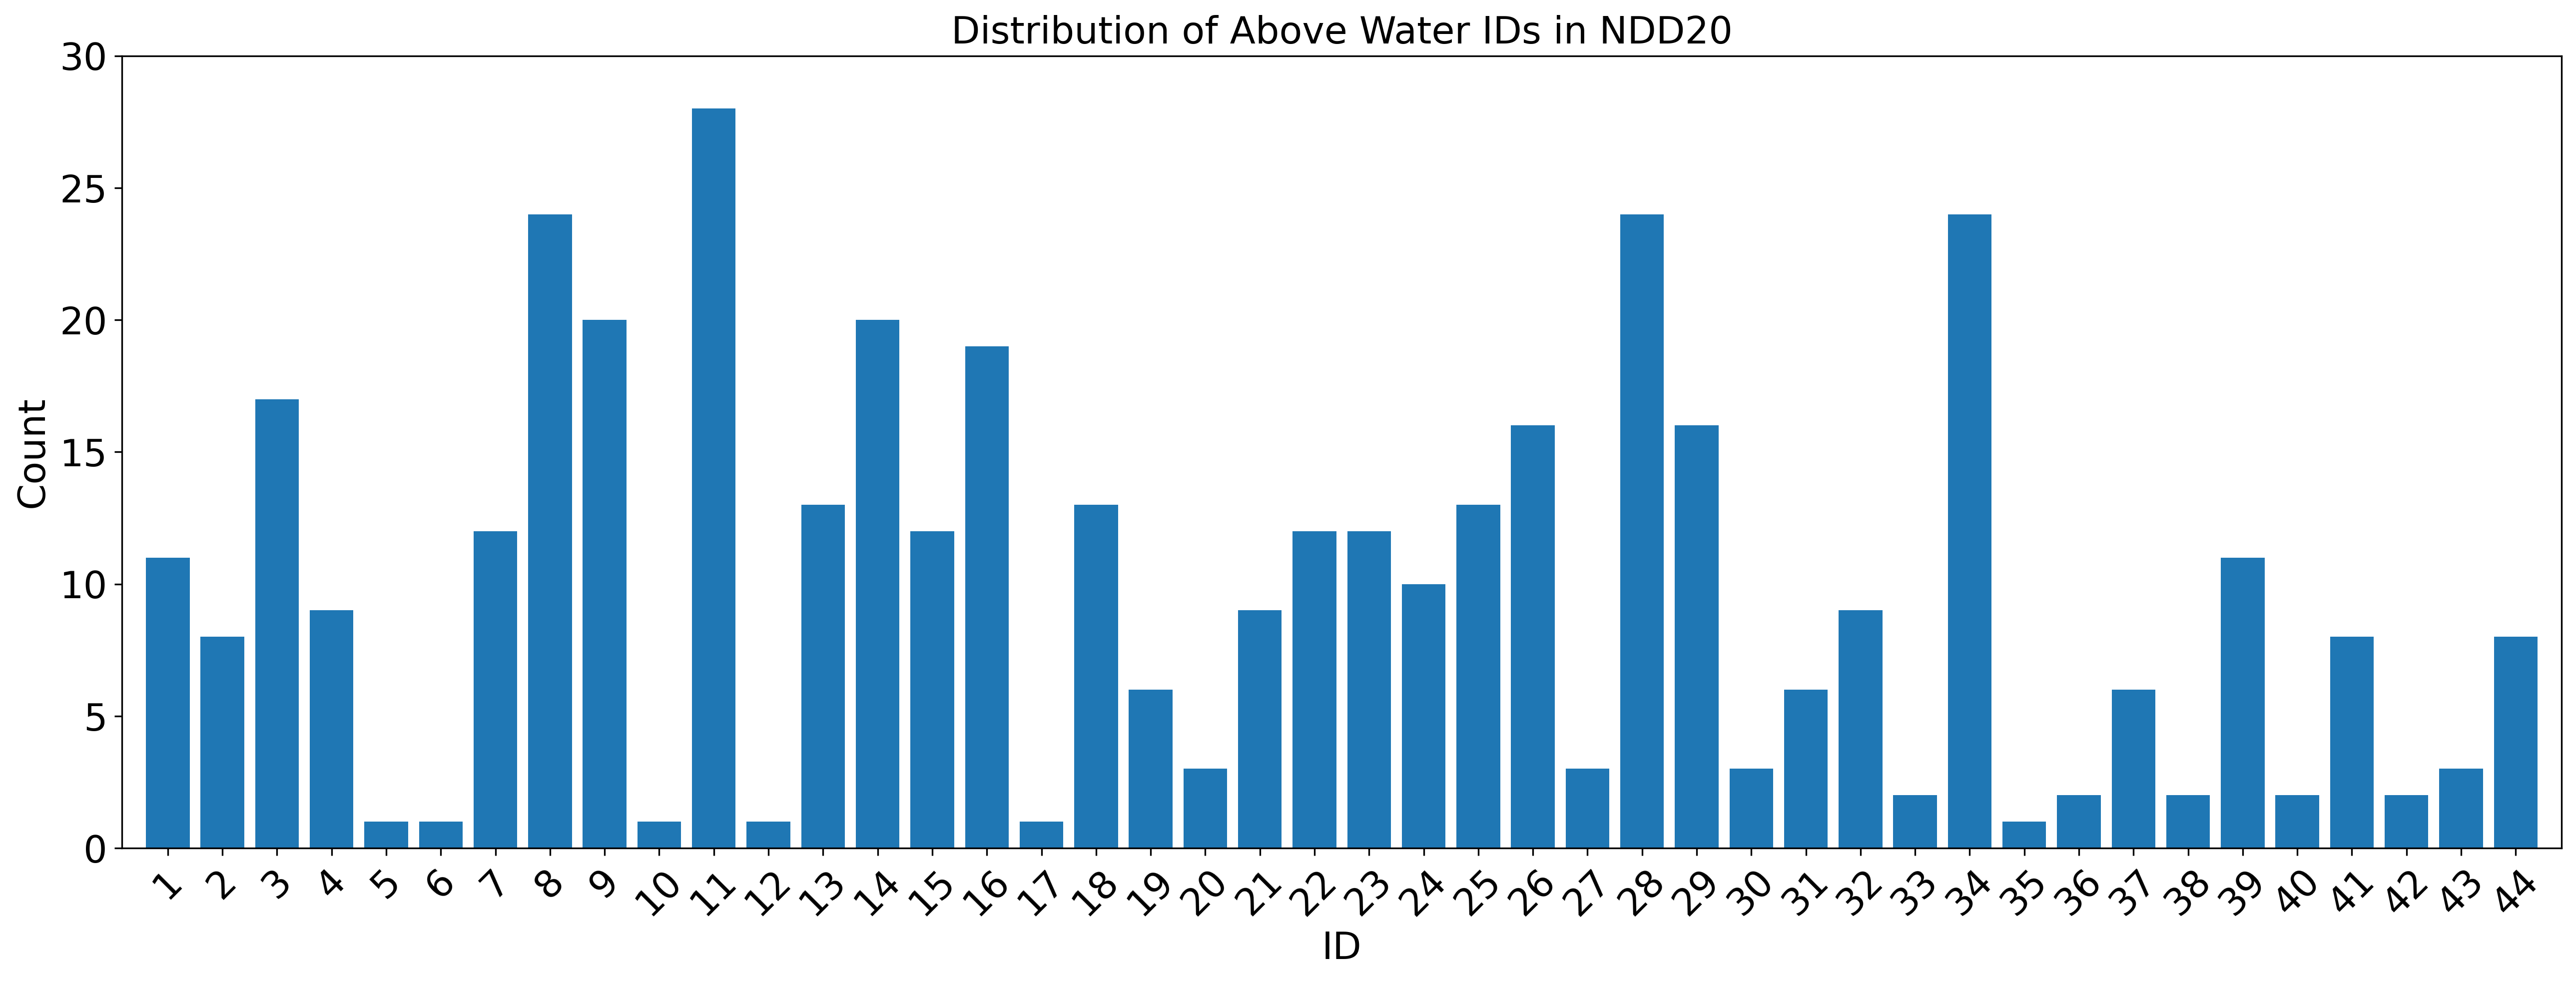
\includegraphics[width=\linewidth]{Chapter3/figs/aboveWaterIDDist_updated.png}
	\end{center}
	\caption{The \texttt{ID} class label distribution for the above water set of NDD20.}
	\label{fig:above-water-id-dist}
\end{figure}

Like its above water counterpart, the below water set also contains 2201 images each with at least one mask containing  a \texttt{dolphin} label. Masks in the below water set are significantly larger than in the above water set, as far more of the cetacean is visible when captured below the waterline. Unlike the above water set however, all below water images also contain at least one mask with an \texttt{ID} class label, with 82 classes represented. The distribution of \texttt{ID} class labels in the below water set can be seen in Figure \ref{fig:below-water-id-dist}. This set represents a significantly more challenging fine-grained and few-show learning problem, both due to the higher number of classes as well as decreased image quality thanks to the nature of underwater photography. The main challenges are water clarity, affected by factors such as algal bloom and sunlight refraction which may both obscure areas of the individual useful for identification or add artificial markings which may hinder this. 

\begin{figure}
	\begin{center}
		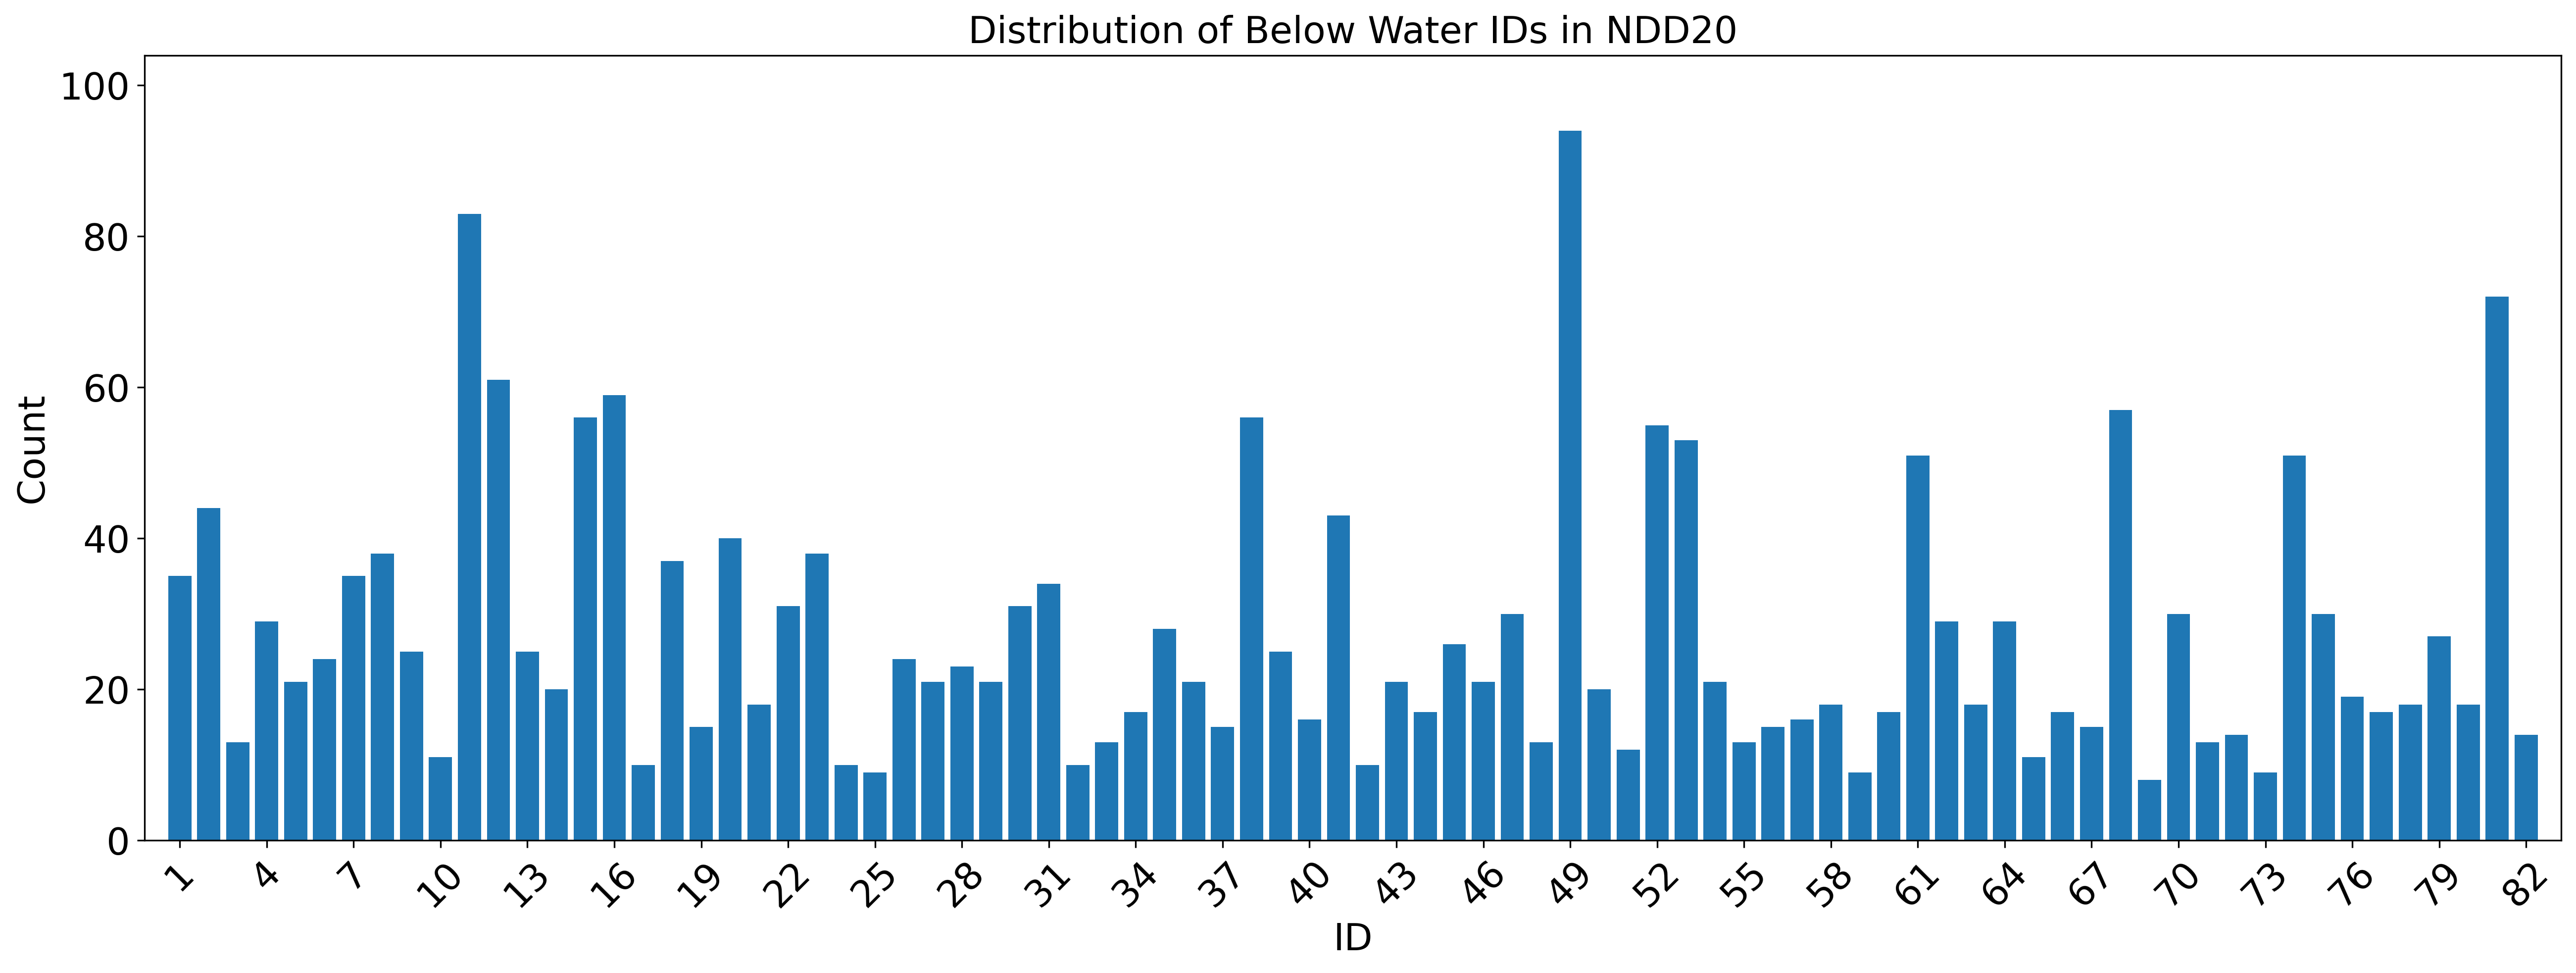
\includegraphics[width=\linewidth]{Chapter3/figs/belowWaterIDDist_updated.png}
	\end{center}
	\caption{The \texttt{ID} class label distribution for the below water set of NDD20.}
	\label{fig:below-water-id-dist}
\end{figure}

NDD20 is small compared to traditional benchmarking computer vision datasets such as ImageNet \cite{deng_imagenet:_2009} or those which are domain specific such as iWildcam \cite{beery_iwildcam_2019} or Caltech-UCSD Birds 200 \cite{welinder_caltech-ucsd_2010}. Even when compared to other related non-benchmark marine ecology datasets such as The Fishnet Open Images dataset \cite{kay_fishnet_2021}, SEAMAPD21 \cite{boulais_seamapd21_2021}, or FathomNet \cite{katija_fathomnet_2022}, the number of images in NDD20 is much lower. Whilst it may be tempting to solely compare NDD20 to the above datasets however, it is important to note the difference in use-case. NDD20 is not designed for use as a large scale dataset for model pre-training like those considered benchmark. In contrast to the non-benchmark ecology datasets mentioned, NDD20 contains class labels which allow for more fine-grained classification. As such, it is better to compare the quality of NDD20 with other individual animal identification datasets.

\begin{table}
	\caption[A comparison of computer vision datasets capable of training models for individual animal identification, sorted by number of individuals.]{A comparison of computer vision datasets capable of training models for individual animal identification, sorted by number of individuals.}\label{tab:animal-id-datasets-comparison}
	\begin{adjustbox}{width=\columnwidth, center}
		\begin{tabular}{*{4}{c}}
			\toprule
			\textbf{Dataset}                                                                                                                         & \textbf{Species}                                                                                                & \textbf{Number of Images} & \textbf{Number of Individuals}  \\
			\midrule
			Beluga ID 2022$^\dagger$ & Beluga whale (\textit{Delphinapterus leucas})                & 5902                      & 788                         \\
			Leopard ID 2022$^\ddagger$ & African leopard (\textit{Panthera pardus})                   & 6795                      & 430                         \\
			Hyena ID 2022$^\mathsection$  & Spotted hyena (\textit{Crocuta crocuta})                      & 3104                      & 256                         \\
			Cows2021 \cite{gao_towards_2021}                                                                                                         & Holstein-Friesian cow (\textit{Bos taurus taurus})    & 10,402                     & 186                         \\
			BearID \cite{clapham_automated_2020}                                                                                                     & Brown bear (\textit{Ursus arctos})                            & 4675                      & 132                         \\
			Multi Camera Pig Tracking \cite{shirke_tracking_2021}                                                                                    & Domestic pig (\textit{Sus scrofa domesticus})                 & 380                       & 33                          \\
			Jaguar ID \cite{timm_large-scale_2018}                                                                                                   & Jaguar (\textit{Panthera onca})                               & 176                       & 16                          \\\midrule
			\multirow{2}{*}{\textbf{NDD20 (Above Water)}}                                                                                                    & Bottlenose dolphin (\textit{Tursiops truncatus})              & \multirow{2}{*}{2201}     & \multirow{2}{*}{44}         \\
			& \& white-beaked dolphin (\textit{Lagenorhynchus albirostris}) &                           &                             \\
			\textbf{NDD20 (Below Water)}                                                                                                                      & White-beaked dolphin (\textit{Lagenorhynchus albirostris})    & 2201                      & 82                         \\
			\bottomrule
		\end{tabular}
	\end{adjustbox}
	
	{\raggedright\footnotesize $\dagger$ Beluga ID 2022: \href{https://lila.science/datasets/beluga-id-2022/}{lila.science/datasets/beluga-id-2022} \\ $\ddagger$ Leopard ID 2022: \href{https://lila.science/datasets/leopard-id-2022/}{lila.science/datasets/leopard-id-2022} \\$\mathsection$ Hyena ID 2022: \href{https://lila.science/datasets/hyena-id-2022/}{lila.science/datasets/hyena-id-2022} \par}
\end{table}

Unlike other datasets for individual animal identification, NDD20 is unusual in that it covers two species. Other ecology datasets that cover a range of species do not include individual identification labels \cite{beery_iwildcam_2019, van_horn_inaturalist_2018, khosla_novel_2011}. This combination of multiple species and individual class labels provides novelty to NDD20. As seen in Table \ref{tab:animal-id-datasets-comparison}, whilst NDD20 is not the smallest dataset available for individual animal identification it is still on the lower end both in terms of number of images and individuals. This is due to the nature of the populations surveyed. The Coquet to St. Mary's and Farnes Deep MCZs are small geographic areas, resulting in smaller population catalogues. 

\section{Summary}\label{ch:datasetCreation,sec:summary}

This chapter explores the creation of two datasets required for further work undertaken in this thesis to be performed. The first, known as the Zanzibar dataset, was developed utilising existing imagery collected by Newcastle University's Marine MEGAfauna Lab and contains coarse-grained labels useful for the creation of an instance segmentation model. The second, known as the Northumberland Dolphin Dataset 2020 (NDD20), was developed through the use of imagery collected during fieldwork undertaken as part of this thesis. Containing both coarse and fine-grained labels, NDD20 provides the data required for both instance segmentation and few-shot classification tasks. The usefulness of NDD20 is highlighted through its inclusion in a publicly hosted Kaggle competition\footnote{Kaggle competition: \href{https://www.kaggle.com/c/happy-whale-and-dolphin/}{kaggle.com/c/happy-whale-and-dolphin}}, acceptance to the 7\textsuperscript{th} Fine-Grained Visual Categorization Workshop (FGVC7) hosted at CVPR 2020 \cite{trotter_ndd20_2020}, and its use in the evaluation of zero-shot segmentation models such as Segment Anything \cite{kirillov_segment_2023}. This highlights the usefulness of NDD20 irrespective of size limitations. 

The use of the Zanzibar dataset to train and evaluate a model capable of instance segmentation of cetaceans in photo-id data, as well as the post-processing of model output images, is explored in Chapter \ref{ch:cetDet}, alongside the use of the NDD20 dataset to evaluate model performance on photo-id data collected of a different species of interest and over a different spatio-temporal scale.
